% RLC main.tex Version 2024.2

\documentclass[10pt]{article} % For LaTeX2e
\usepackage{rlc}
\usepackage{amsmath}

% If accepted, instead use the following line for the camera-ready submission:
%\usepackage[accepted]{rlc}
% To de-anonymize and remove mentions to RLC (for example, for posting to preprint servers), instead use the following:
% \usepackage[preprint]{rlc}

%%%%%%%%%%%%%%%%%%%%%%%%%%%%%%%%%%%%%%%%%%%%%%%%%%%%%%%%%%%%%%%%
%% Recommended (but not required) packages
%%%%%%%%%%%%%%%%%%%%%%%%%%%%%%%%%%%%%%%%%%%%%%%%%%%%%%%%%%%%%%%%
\usepackage{amssymb}            % Defines common symbols like \mathbb R
\usepackage{mathtools}          % Extends amsmath, providing common math tools
\usepackage{mathrsfs}           % Enables \mathscr, which can work in cases that \mathcal does not
\mathtoolsset{showonlyrefs}     % Only number equations that are referenced (optional)
\usepackage{graphicx}           % For including images
\usepackage{subcaption}         % Allows for the use of subfigures and subcaptions
\usepackage[space]{grffile}     % For spaces in image names
\usepackage{url}                % For displaying urls

%%%%%%%%%%%%%%%%%%%%%%%%%%%%%%%%%%%%%%%%%%%%%%%%%%%%%%%%%%%%%%%%
%% Title Page Specification
%%%%%%%%%%%%%%%%%%%%%%%%%%%%%%%%%%%%%%%%%%%%%%%%%%%%%%%%%%%%%%%%
\title{Models of the thesis}

% Authors must not appear in the submitted version. They should be hidden
% as long as the tmlr package is used without the [accepted] or [preprint] options.
% Non-anonymous submissions will be rejected without review.

\author{Philip S. Thomas  \\
    pthomas@cs.umass.edu \\
    College of Information and Computer Sciences\\
    University of Massachusetts
    \And
    Glen Berseth \\
    glen.berseth@mila.quebec\\
    Mila, Universit\'e de Montr\'eal \\
    CIFAR Canada AI Chair}

% The \author macro works with any number of authors. Use \AND 
% to\ separate the names and addresses of multiple authors.

%%%%%%%%%%%%%%%%%%%%%%%%%%%%%%%%%%%%%%%%%%%%%%%%%%%%%%%%%%%%%%%%
%% Begin document, create title and abstract
%%%%%%%%%%%%%%%%%%%%%%%%%%%%%%%%%%%%%%%%%%%%%%%%%%%%%%%%%%%%%%%%
\begin{document}
    \bibliographystyle{plain}  % Scegli uno stile adatto
    
    \section{Information about the dataset and pre-processing}
    From here until the end of this report, only the stations that measure the '$AQ\_nh3$' variable were selected and used (i.e. the stations that measure ammonia), in total there are 10. Subsequently, the station with the same 'IDStations' parameter was used to 1266, that correspond to Bertonico Via Moro station.
    
    As pre-processing it was done a standardization described in the equation \ref{eq:normalization}.
      \begin{equation}
        X_{standardized} = \frac{X-\mu}{\sigma}
        \label{eq:normalization} 
    \end{equation}
    \\For all models both x and y were divided into train sets and test sets with a 70-30 split (70\% train and 30\% test).

    \subsection{Two steps approach for neural networks}
    Using a two-step sieve approach, hyperparameters were carefully selected for the neural network-based models. Initially, a comprehensive exploration was conducted, considering all possible combinations of hyperparameters. Subsequently, to refine the search space, an interval with a smaller delta was chosen, ensuring a finer granularity in parameter tuning. The hyperparameters under investigation included the configuration of the hidden layer (\texttt{units\_hidden\_layer}), with options ranging from 64 to 256 neurons. The learning rate (\texttt{learning\_rate}) was systematically varied across a spectrum of values, encompassing 0.001, 0.01, and 0.1. Furthermore, the range for the number of iterations (\texttt{num\_iterations\_range}) was meticulously explored, spanning from 10 to 40, to ascertain the optimal training regimen. Similarly, the number of epochs (\texttt{num\_epochs\_range}) was examined across a breadth of values, ranging from 200 to 500, ensuring a thorough exploration of the training process. This rigorous and systematic approach to hyperparameter tuning aimed to maximize the model's performance, robustness, and generalizability across diverse datasets and tasks.
    \\For the neural network based models the initial values are:

     \begin{itemize}
        \item units\_hidden\_layer = [64, 128, 256]
        \item learning\_rate = [0.001, 0.01, 0.1]
        \item num\_iterations\_range = [10, 20, 30, 40]
        \item num\_epochs\_range = [200, 300, 400, 500]
    \end{itemize}
    \section{Linear regression}
    \subsection{Description of the model}
    Linear regression is a fundamental statistical technique utilized to model relationships between dependent and independent variables. In simple linear regression, we examine the association between a single independent variable and the dependent variable, assuming a linear relationship. This model is expressed as \(Y = \beta_0 + \beta_1 X + \epsilon\), where \(Y\) is the dependent variable, \(X\) is the independent variable, \(\beta_0\) is the intercept, \(\beta_1\) is the slope, and \(\epsilon\) represents the error term. Multiple linear regression extends this concept to incorporate multiple independent variables, enabling the analysis of more complex relationships. Here, the model becomes \(Y = \beta_0 + \beta_1 X_1 + \beta_2 X_2 + \ldots + \beta_k X_k + \epsilon\), where \(X_1, X_2, \ldots, X_k\) are the independent variables, and \(\beta_0, \beta_1, \ldots, \beta_k\) are the corresponding coefficients. Both simple and multiple linear regression models are estimated using techniques such as ordinary least squares (OLS) to minimize the sum of squared errors, providing valuable insights into the relationships within data and facilitating predictive analysis.


    \subsection{Results for the simple linear regression model}
    The regression results indicate the performance of a linear regression model on different datasets: training set, validation set, and test set. 

\begin{itemize}
  \item \textbf{Training Set Metrics}: The mean absolute error (MAE) on the training set is 0.05, indicating that, on average, the model's predictions deviate from the actual values by 0.05 units. The R-squared value (0.68) suggests that 68\% of the variance in the dependent variable is explained by the independent variables included in the model. The root mean squared error (RMSE) is 0.08, indicating the average magnitude of the errors in the model's predictions.
  
  \item \textbf{Validation Set Metrics}: The MAE on the validation set is slightly higher at 0.07, indicating a slightly worse performance compared to the training set. The R-squared value (0.52) is lower than that of the training set, suggesting that the model might be overfitting to the training data. The RMSE and MSE values provide additional measures of the error in the model's predictions on the validation set.
  
  \item \textbf{Test Set Metrics}: The MAE on the test set is the same as that of the training set at 0.05, suggesting consistent performance between the two sets. The R-squared value (0.64) falls between the values of the training and validation sets, indicating reasonable generalization performance. The RMSE and MSE values are also provided for assessing the model's performance on the test set.
  
\end{itemize}
    \section{Plain neural network}
    \subsection{Description of the model}
    Neural networks, inspired by the intricate structure and functionality of the human brain, represent a fundamental class of machine learning algorithms. At their core lies the artificial neuron, a computational unit that takes multiple inputs, each weighted by a parameter, and produces an output using an activation function. These neurons are organized into layers within the neural network, with each layer responsible for processing and transforming the data in increasingly abstract ways. During the training process, the network learns from labeled data by adjusting the weights and biases of the neurons to minimize the difference between predicted and actual outputs, typically through optimization algorithms like gradient descent. This iterative process allows the neural network to generalize patterns and make accurate predictions on unseen data. The applications of neural networks span across various domains, including image and speech recognition, natural language processing, autonomous vehicles, and healthcare, where they have demonstrated remarkable success in tasks ranging from image classification to medical diagnosis. Understanding the fundamentals of neural networks is crucial for leveraging their power in real-world applications and driving further advancements in artificial intelligence and machine learning technologies.
    Neural networks, inspired by the intricate structure and functionality of the human brain, represent a fundamental class of machine learning algorithms. At their core lies the artificial neuron, modeled mathematically as $y = f\left(\sum_{i=1}^{n} w_i \cdot x_i + b\right)$, where $x_i$ represents the input, $w_i$ denotes the corresponding weight, $b$ is the bias, and $f$ is the activation function. These neurons are organized into layers within the neural network, with each layer responsible for processing and transforming the data in increasingly abstract ways. During the training process, the network learns from labeled data by adjusting the weights and biases to minimize the difference between predicted and actual outputs, typically through optimization algorithms like gradient descent. This iterative process allows the neural network to generalize patterns and make accurate predictions on unseen data. The applications of neural networks span across various domains, including image and speech recognition, natural language processing, autonomous vehicles, and healthcare, where they have demonstrated remarkable success in tasks ranging from image classification to medical diagnosis. Understanding the fundamentals of neural networks is crucial for leveraging their power in real-world applications and driving further advancements in artificial intelligence and machine learning technologies.
      
    \subsection{Result for the first iteration}

    Best Model Metrics for test:
    \begin{itemize}
        \item Best MAE: 0.25
        \item Best R-squared (R2): 0.25
        \item Best RMSE: 0.28
    \end{itemize}

Best Hyperparameters for the Best Model:

    \begin{itemize}
        \item Number of Epochs: 300
        \item Number of Iterations: 30
        \item Units Hidden Layer: 64
        \item Learning Rate: 0.001
        \item Training Time for Best Model: 3.25 seconds
    \end{itemize}

    \begin{figure}
        \centering
        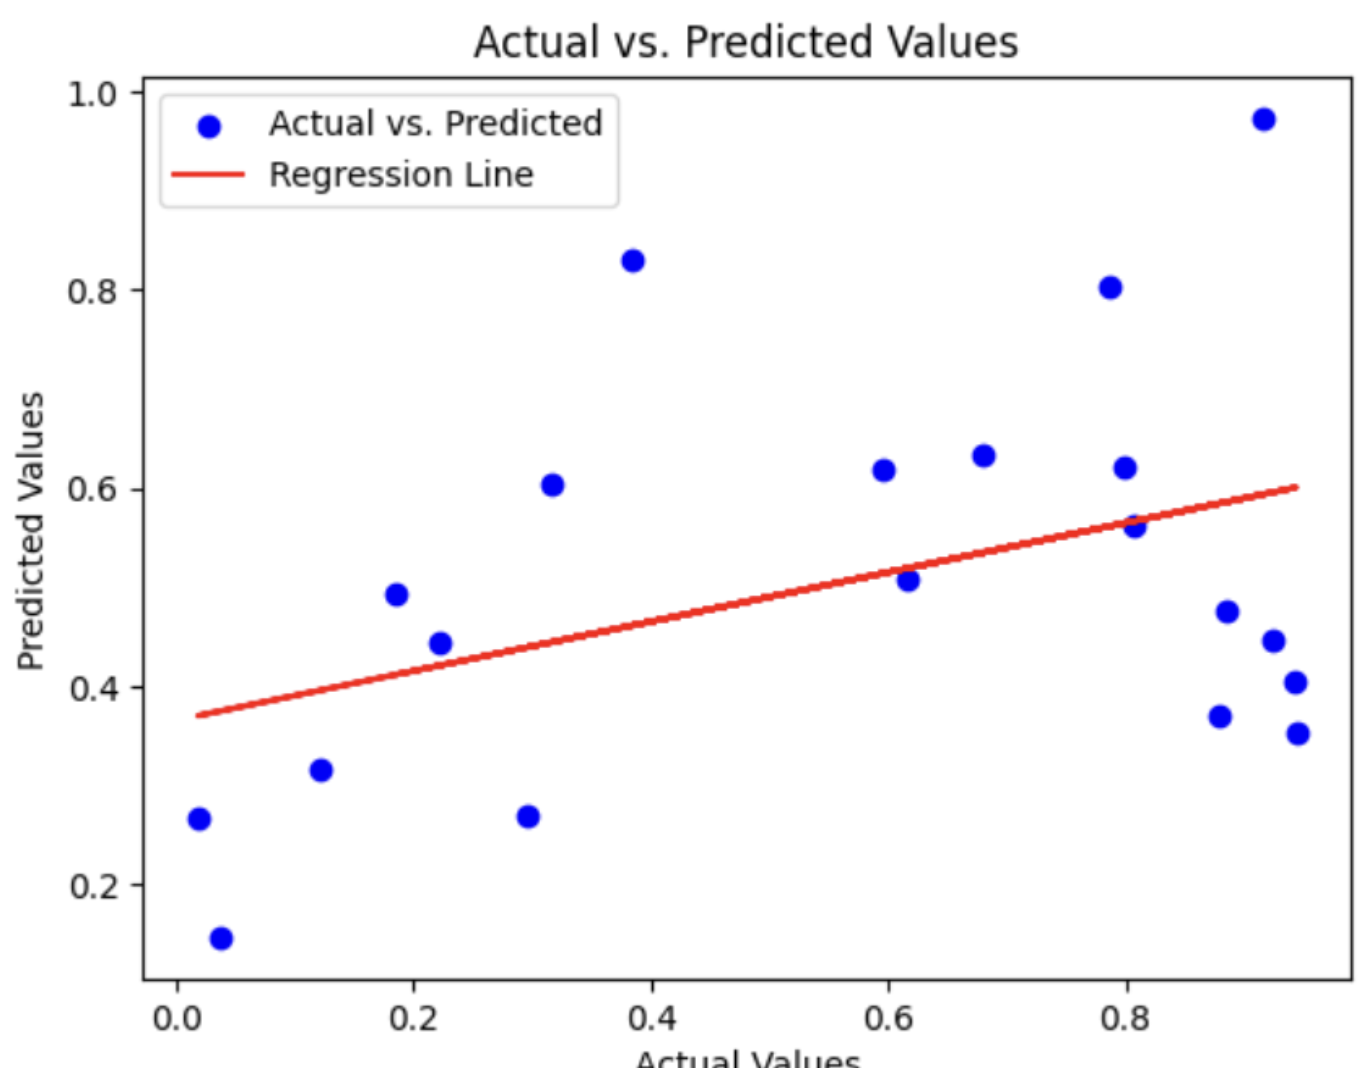
\includegraphics[scale=0.4]{Assets/iteration 1/nn_it1_1.png}
        \caption{Time series for neural network result for the first iteration}
        \label{fig:enter-label}
    \end{figure}

    \begin{figure}
        \centering
        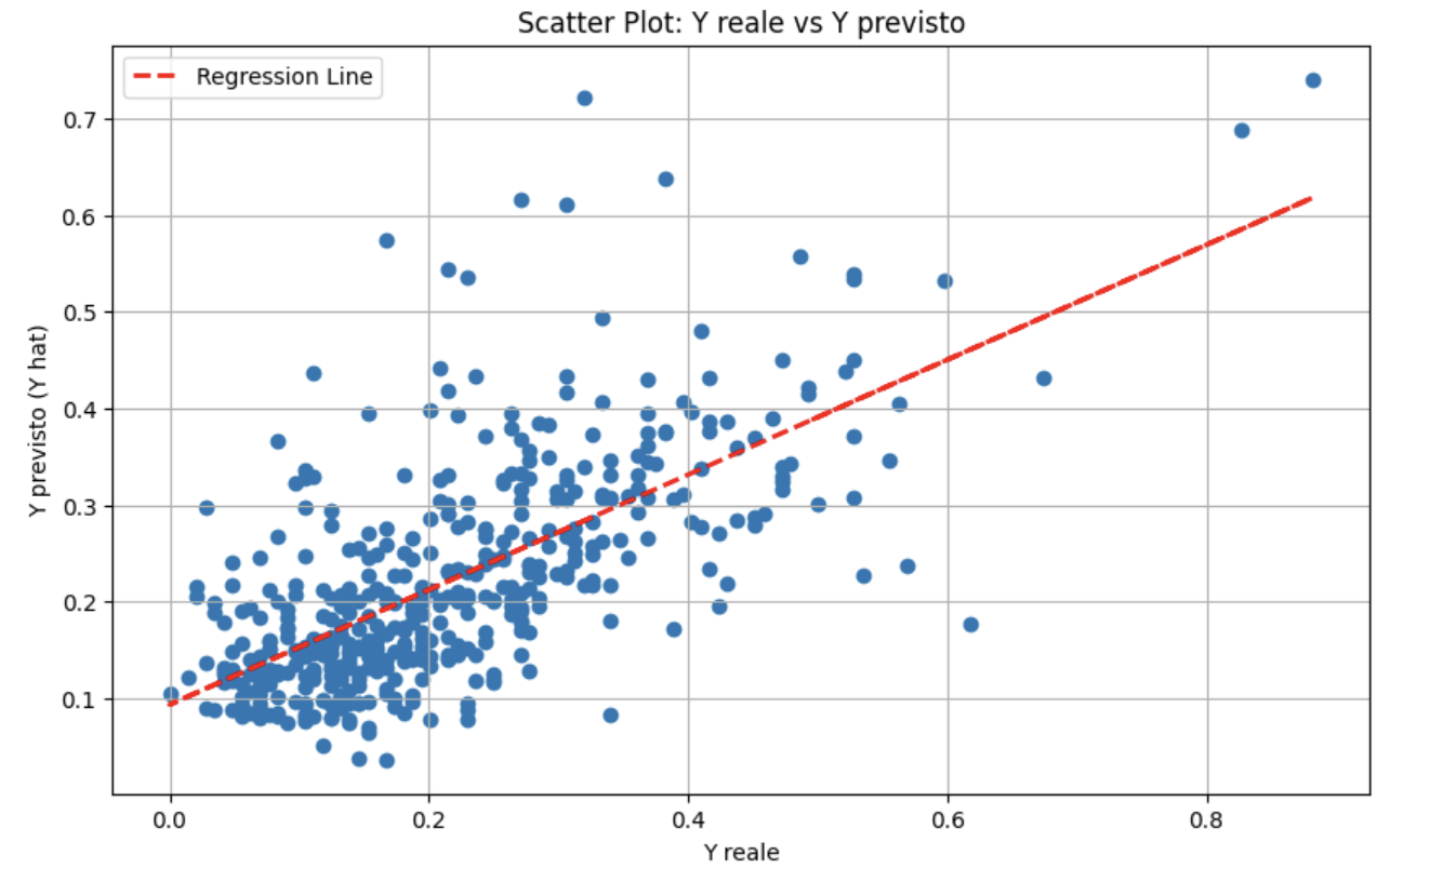
\includegraphics[scale=0.4]{Assets/iteration 1/rnn_it1_2.png}
        \caption{$\hat{y}$ vs. y\_real for neural network model for the first iteration}
        \label{fig:enter-label}
    \end{figure}

    \newpage
    \subsection{Results for the second iteration}

    The new starting parameters for the model are:
    \begin{itemize}
        \item  units\_hidden\_layer = [0, 32, 64, 96, 128]
        \item learning\_rates = [0.001, 0.01, 0.1]
        \item num\_iterations\_range = [20 ,25, 30, 35, 40]
        \item num\_epochs\_range = [250, 300, 350, 400]
    \end{itemize}

Best Model Metrics training:
    \begin{itemize}
        \item Best MAE: 0.24

        \item Best R-squared (R2): 0.14

        \item Best RMSE: 0.29

    \end{itemize}
    Best Hyperparameters for the Best Model:
    \begin{itemize}
        \item Number of Epochs: 250
        \item Number of Iterations: 10
        \item Units Hidden Layer: 192
        \item Learning Rate: 0.01
        \item Training Time for Best Model: 20.158 seconds
    \end{itemize}
    The results indicate a thorough exploration of hyperparameters, including varying units in hidden layers, learning rates, number of iterations, and epochs. 
    \\It's interesting to observe the impact of these parameters on model performance metrics such as Mean Absolute Error (MAE), R-squared (R2), and Root Mean Squared Error (RMSE).
    \\Despite the extensive search, the best model achieved a MAE of 0.24, R2 of 0.14, and RMSE of 0.29, which suggests that there might be room for improvement.
    Notably, the best model was trained with 250 epochs, 10 iterations, 192 units in the hidden layer, and a learning rate of 0.01. 
    \\The training time for this model was 20.158 seconds, indicating a reasonable computational cost for the achieved performance.

    \begin{figure}
        \centering
        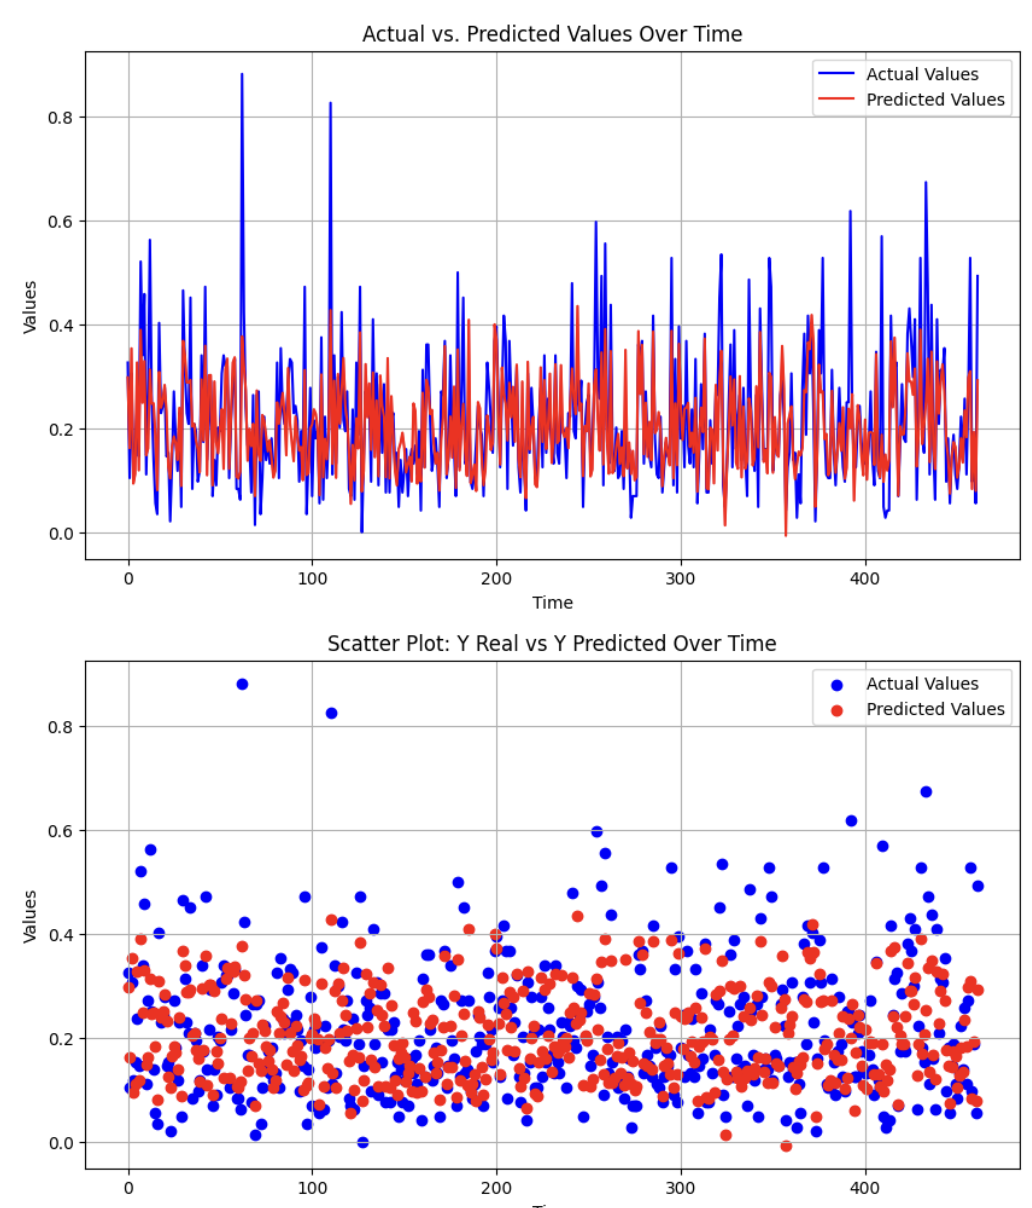
\includegraphics[scale=0.4]{Assets/iteration 2/rnn_it2_1.png}
        \caption{Time series for neural network result for the second iteration}
        \label{fig:enter-label}
    \end{figure}

    \begin{figure}
        \centering
        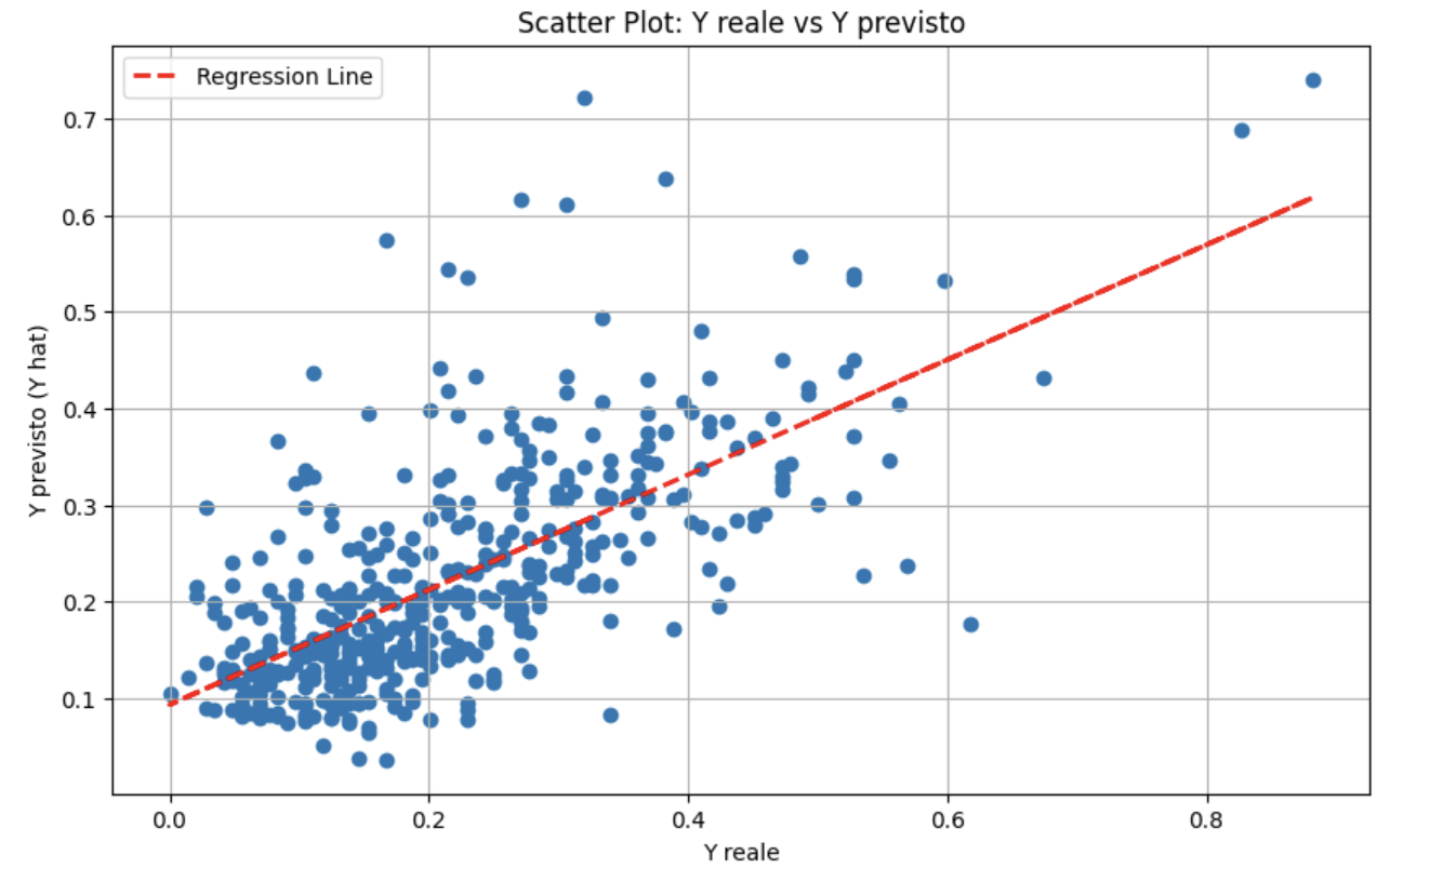
\includegraphics[scale=0.4]{Assets/iteration 1/rnn_it1_2.png}
        \caption{$\hat{y}$ vs. y\_real for neural network model for the second iteration}
        \label{fig:enter-label}
    \end{figure}
    \newpage

    \section{Recurrent Neural Network (RNN)}
    \subsection{Description of the model}
    Recurrent Neural Networks (RNNs) are a class of artificial neural networks designed for sequence modeling tasks. Unlike feedforward neural networks, which process input data independently, RNNs maintain an internal state that captures information about previous inputs. This recurrent nature enables RNNs to effectively handle sequential data such as time series, natural language, and audio signals. The key feature of RNNs is their ability to exhibit dynamic temporal behavior, making them suitable for tasks requiring context and memory. However, traditional RNN architectures suffer from vanishing or exploding gradient problems, limiting their ability to capture long-range dependencies. To address these issues, various RNN variants have been proposed, including Long Short-Term Memory (LSTM) and Gated Recurrent Unit (GRU) networks, which incorporate mechanisms to alleviate gradient vanishing and exploding problems. These advancements have significantly improved the performance of RNNs, making them a cornerstone in many machine learning applications.

    \subsection{Results for the first iteration}

    Best Model Metrics testing:
    \begin{itemize}
        \item     Best MAE: 0.07
        \item Best R-squared (R2): 0.45 
        \item Best RMSE: 0.1
    \end{itemize}

Best Hyperparameters for the Best Model:

    \begin{itemize}
        \item Number of Epochs: 300
        \item Number of Iterations: 20
        \item Units Hidden Layer: 256
        \item Learning Rate: 0.001
        \item Training Time for Best Model: 20.26 seconds
    \end{itemize}
    The testing metrics for the best RNN model demonstrate promising performance, with a low Mean Absolute Error (MAE) of 0.07, a relatively high R-squared (R2) value of 0.45, and a small Root Mean Squared Error (RMSE) of 0.1.
    \\These metrics indicate that the model has effectively captured patterns and relationships within the data.
    \\The hyperparameters chosen for the best model include 300 epochs, 20 iterations, 256 units in the hidden layer, and a learning rate of 0.001.
    \\Despite the complexity of the model, the training time remains reasonable at 20.26 seconds, suggesting efficient training procedures.
    \\Overall, these results suggest that the RNN architecture, when tuned appropriately, can yield strong predictive performance on the given task.
    
    \begin{figure}
        \centering
        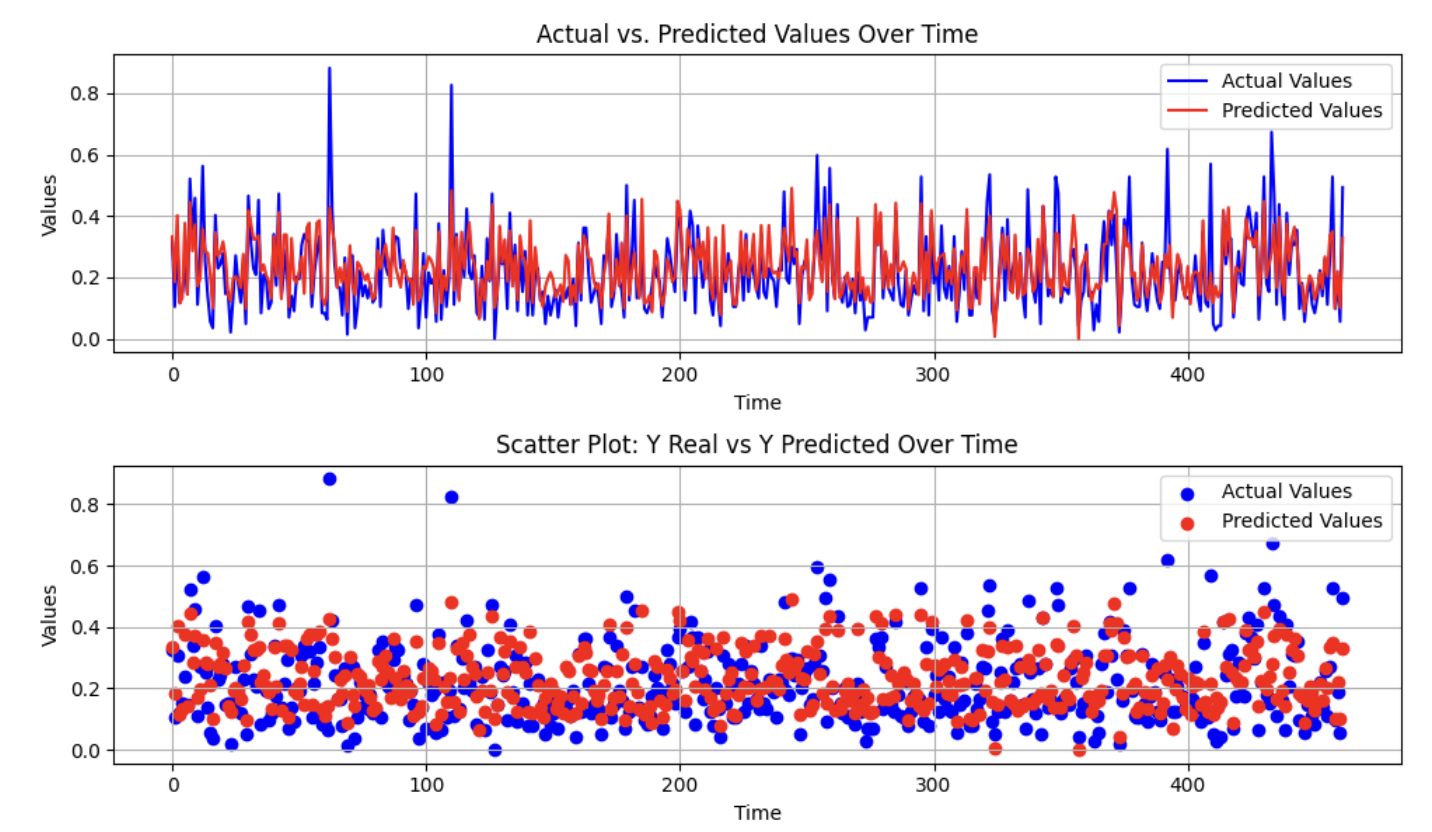
\includegraphics[scale = 0.4]{Assets/iteration 1/lstm_it1_1.png}
        \caption{Time series for the recurrent neural network result for the first iteration}
        \label{fig:enter-label}
    \end{figure}
    
    \begin{figure}
        \centering
        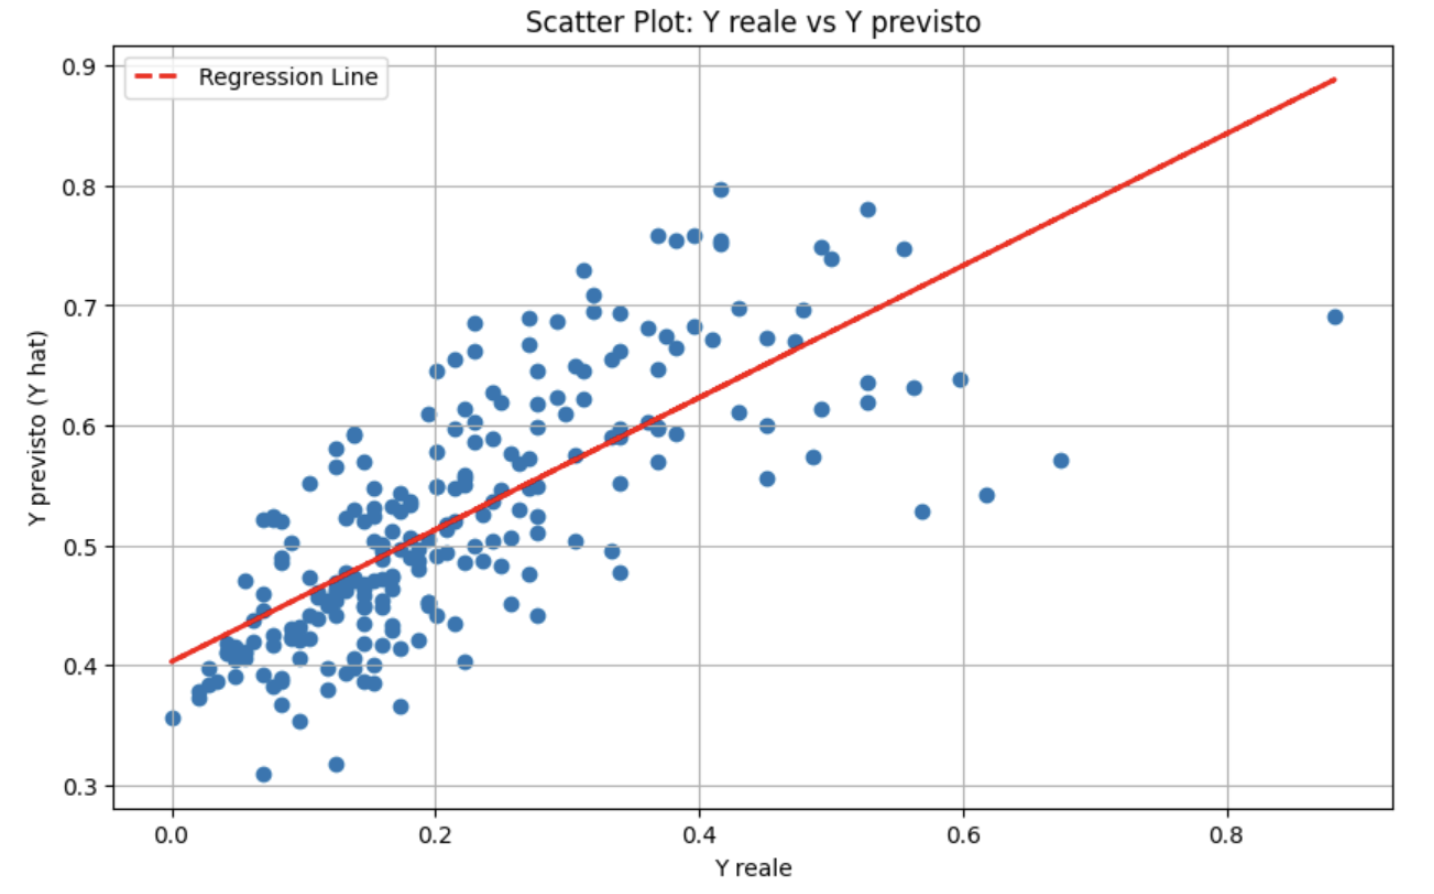
\includegraphics[scale = 0.4]{Assets/iteration 1/lstm_it1_2.png}
        \caption{$\hat{y}$ vs. y\_real for the recurrent neural network model for the second iteration}
        \label{fig:enter-label}
    \end{figure}
    \newpage

    \subsection{Results for the second iteration}
      The new starting parameters for the model are:
    \begin{itemize}
        \item  units\_hidden\_layer = [192, 224, 256, 288, 320]
        \item learning\_rates =  [0.001, 0.01, 0.1]
        \item num\_iterations\_range = [10, 15, 20, 25, 30]
        \item num\_epochs\_range = [200, 250, 300, 350, 400]
    \end{itemize}
    
    Best Model Metrics training:
    \begin{itemize}
        \item Best MAE: 0.06
        \item Best R-squared (R2): 0.58
        \item Best RMSE: 0.08
    \end{itemize}
    Best Hyperparameters for the Best Model:
    \begin{itemize}
        \item Number of Epochs: 350
        \item Number of Iterations: 25
        \item Units Hidden Layer: 288
        \item Learning Rate: 0.01
        \item Training Time for Best Model: 20.158 seconds
    \end{itemize}

    \section{Long Short Term Memory (LSTM)}
    \subsection{Description of the model}
    Long Short-Term Memory (LSTM) networks are a type of recurrent neural network (RNN) architecture specifically designed to address the vanishing and exploding gradient problems encountered in traditional RNNs. LSTMs are equipped with memory cells that can store information over long periods, allowing them to capture dependencies in sequential data more effectively. Unlike standard RNNs, LSTMs have gated units that regulate the flow of information through the network, consisting of input, forget, and output gates. These gates control the information flow into and out of the memory cells, enabling LSTMs to selectively update and forget information as needed. This architecture enables LSTMs to learn long-range dependencies in sequences, making them particularly well-suited for tasks such as language modeling, machine translation, and speech recognition. Over the years, LSTMs have become a cornerstone in sequential data analysis, demonstrating superior performance compared to traditional RNNs in various applications.

    \subsection{LSTM cell} \label{lstmcell}
The Long Short-Term Memory (LSTM) cell was introduced in 1997 in \citeauthor{LSTM} \autocite{LSTM}.
It offers improved performance and results compared to a other types of cells, such as RNN cells. In fact, LSTM neural networks have shorter convergence times and are also able to keep track of medium to long term dependencies in time series data such as trend and seasonality.

\begin{figure} [h]
    \centering
    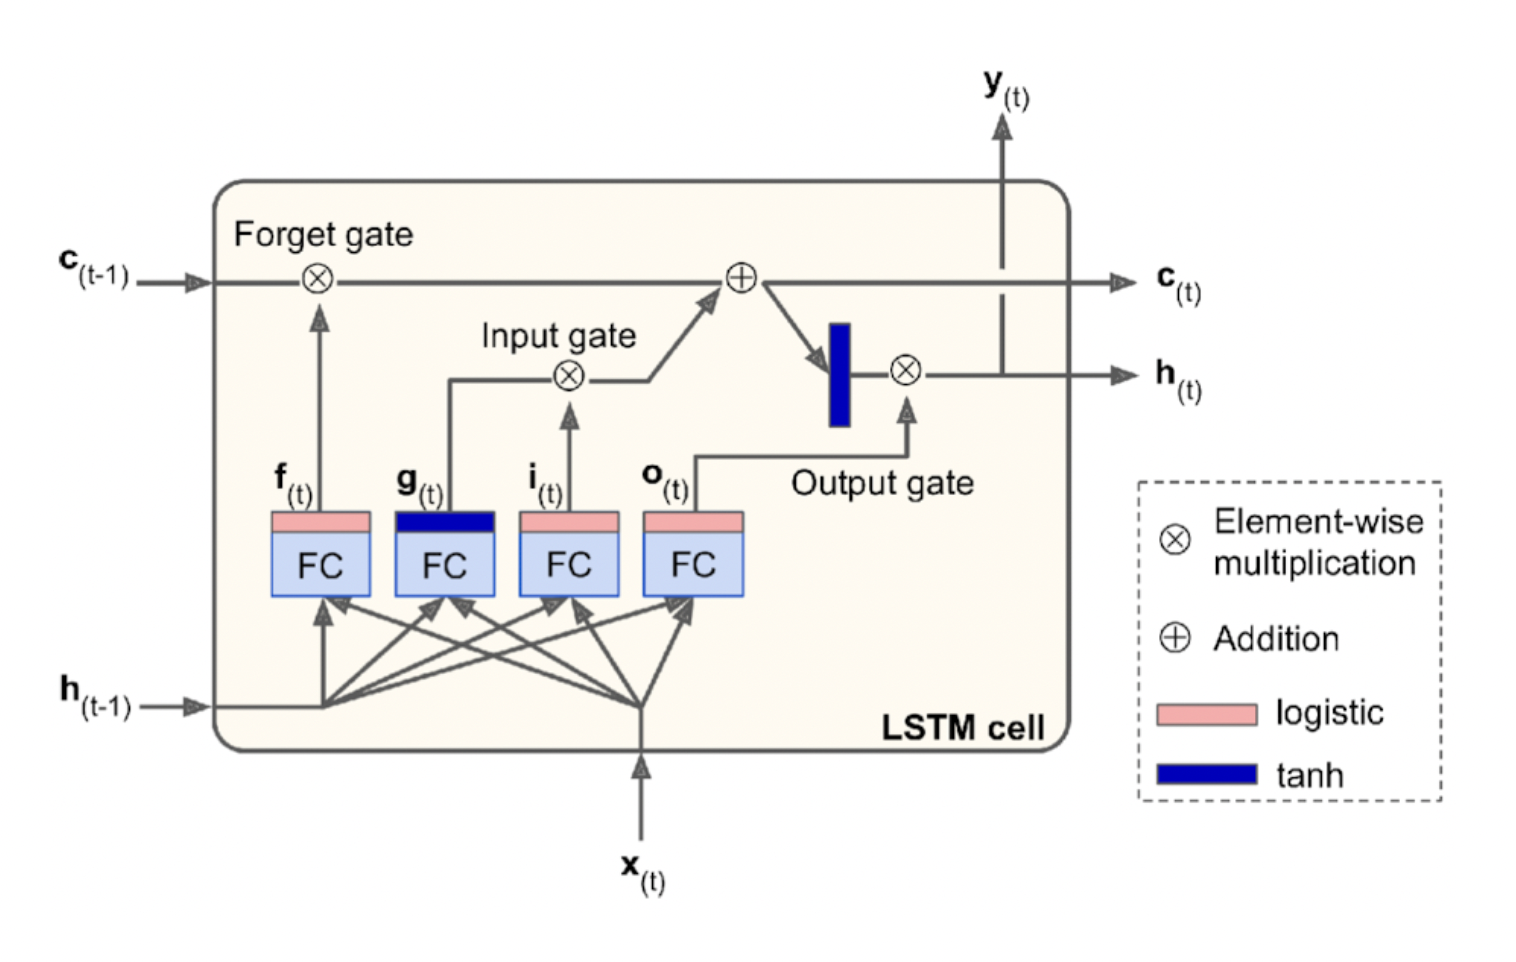
\includegraphics[width=\textwidth,height=\textheight,keepaspectratio]{Assets/Theory_and_method/unnamed-8.png}
    \caption{LSTM cell.}
    \label{fig:LSTM_cell}
\end{figure}

As can be see in figure ~\ref{fig:LSTM_cell}, the cell works exactly like a classic cell, except that the state is split into 2 vectors: ${\bf h}_{(t)}$ and ${\bf c}_{(t)}$, which represent respectively the short term state and the long term state.
\begin{itemize}
    \item The main component is the one that deals with the output ${\bf g}_{(t)}$. Its activation function is a hyperbolic tangent. It deals with analyzing the input ${\bf g} {(t)}$ and the previous state ${\bf h}_{(t-1)}$. In a basic cell this would be the only component and its output would go directly to ${\bf y }_{(t)}$ and ${\bf h} _{(t)}$. In contrast, in LSTM cells the output of this cell is processed such that the most important information in the long-term state is kept and the rest of the data that is not useful is dropped. 
    \item
        The other three components are called gate controllers, because they use the logistic function as the activation function and thus their output range is between 0 and 1. Their roles are as follows: 
        \begin{itemize}
            \item ${\bf f}_{(t)}$ is called the forget gate, which defines which part of the long-term memory is to be erased. 
            \item ${\bf i}_{(t)}$ is the input gate, which determines which part of g (t) should be added to the long-term memory.
            \item ${\bf o}_{(t)}$ is called the output gate and controls which part of long-term memory should be read and added to the output, both for ${\bf h}_{(t)}$ and ${\bf y}_{(t)}$.
        \end{itemize}
\end{itemize}


Therefore, an LSTM cell can learn to recognize particularly important inputs, add them the long-term state, and store them internally until it is needed. This explains why this model has been more successful in capturing long-term patterns when it comes to time series.

 Eq. \eqref{systemformula} contains the mathematical construction of an LSTM cell.

\begin{equation} 
    \begin{array}{l}
    \mathbf{i}_{(t)}=\sigma\left(\mathbf{W}_{x i}^{\top} \mathbf{x}_{(t)}+\mathbf{W}_{h i}^{\top} \mathbf{h}_{(t-1)}+\mathbf{b}_{i}\right) \\
    \mathbf{f}_{(t)}=\sigma\left(\mathbf{W}_{x f}^{\top} \mathbf{x}_{(t)}+\mathbf{W}_{h f}^{\top} \mathbf{h}_{(t-1)}+\mathbf{b}_{f}\right) \\
    \mathbf{o}_{(t)}=\sigma\left(\mathbf{W}_{x o}^{\top} \mathbf{x}_{(t)}+\mathbf{W}_{h o}^{\top} \mathbf{h}_{(t-1)}+\mathbf{b}_{o}\right) \\
    \mathbf{g}_{(t)}=\tanh \left(\mathbf{W}_{x g}^{\top} \mathbf{x}_{(t)}+\mathbf{W}_{h g}^{\top} \mathbf{h}_{(t-1)}+\mathbf{b}_{g}\right) \\
    \mathbf{c}_{(t)}=\mathbf{f}_{(t)} \otimes \mathbf{c}_{(t-1)}+\mathbf{i}_{(t)} \otimes \mathbf{g}_{(t)} \\
    \mathbf{y}_{(t)}=\mathbf{h}_{(t)}=\mathbf{o}_{(t)} \otimes \tanh \left(\mathbf{c}_{(t)}\right)
    \end{array}
    \label{systemformula}
\end{equation}
The meanings of the terms in the equations are as follows:

\begin{itemize}
    \item  ${\bf W}_{xi} , {\bf W}_{xf} , {\bf W}_{x0}$ and $\: {\bf W}_{xg}$ are the matrices that contain the weights for each of the four components with respect to their connection to the input vector ${\bf x}_{(t)}$.
   
    \item ${\bf W}_{hi} , {\bf W}_{hf} , {\bf W}_{h0}$ and ${\bf W}_{hg}$ are the matrices that contain the weights for each of the four components with respect to their connection to the short term memory state ${\bf h}_{(t-1)}$.
    
    \item ${\bf b}_{i} , {\bf b}_{f}, {\bf b}_{0},$  and ${\bf b}_{g}$ are the bias values for each of the four components. 

\end{itemize}

\clearpage



    
    \subsection{Results for the first iteration}

    Best Model Metrics testing:
    \begin{itemize}
        \item Best MAE: 0.061
        \item Best R-squared (R2): 0.59
        \item Best RMSE: 0.082
    \end{itemize}

Best Hyperparameters for the Best Model:

    \begin{itemize}
        \item Number of Epochs: 300
        \item Number of Iterations: 10
        \item Units Hidden Layer: 128
        \item Learning Rate: 0.001,
        \item Training Time for Best Model:  67.73 seconds
    \end{itemize}

    \begin{figure}
        \centering
        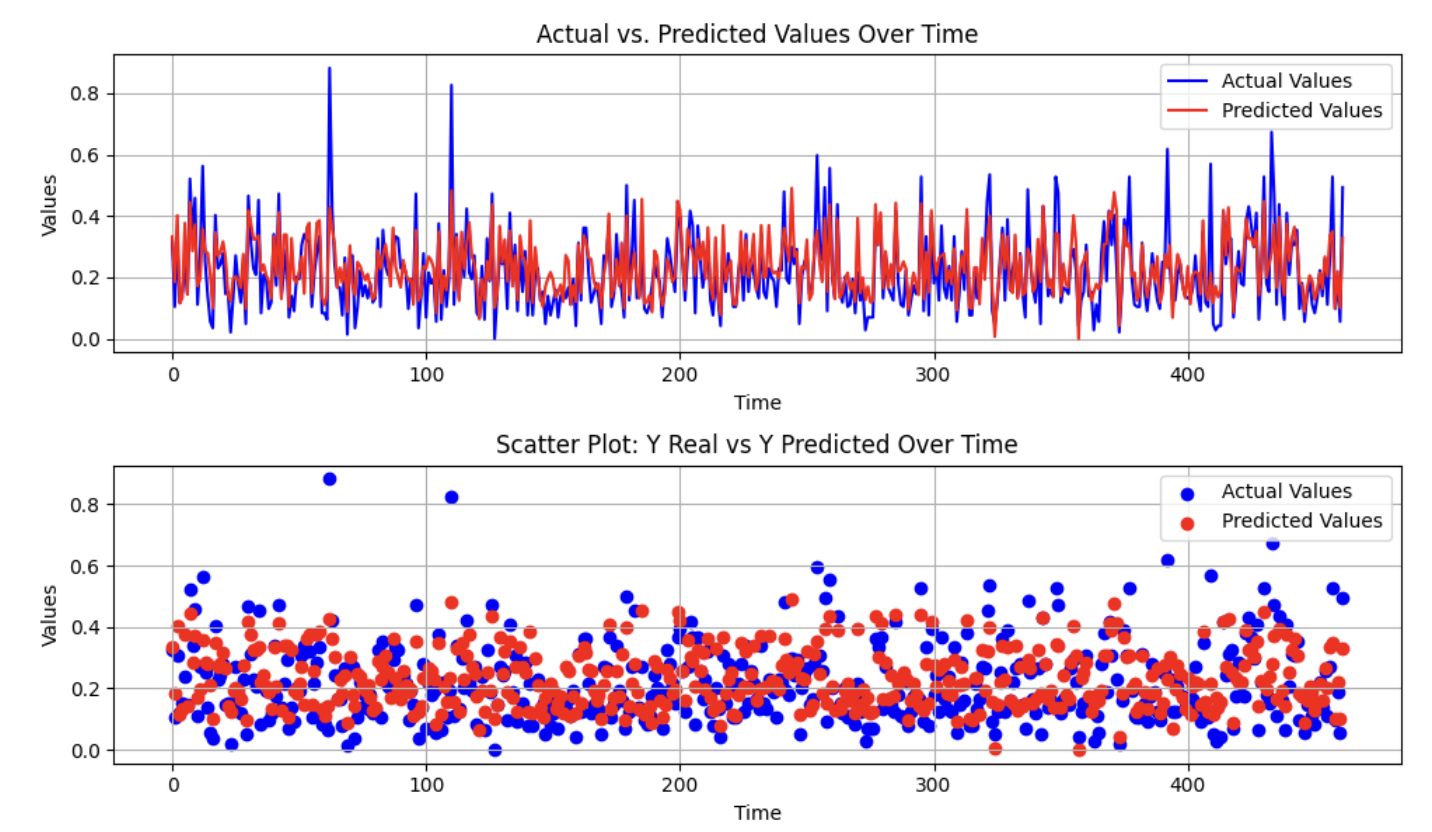
\includegraphics[scale=0.4]{Assets/iteration 1/lstm_it1_1.png}
        \caption{Time series for the LSTM result for the first iteration}
        \label{fig:enter-label}
    \end{figure}

    \begin{figure}
        \centering
        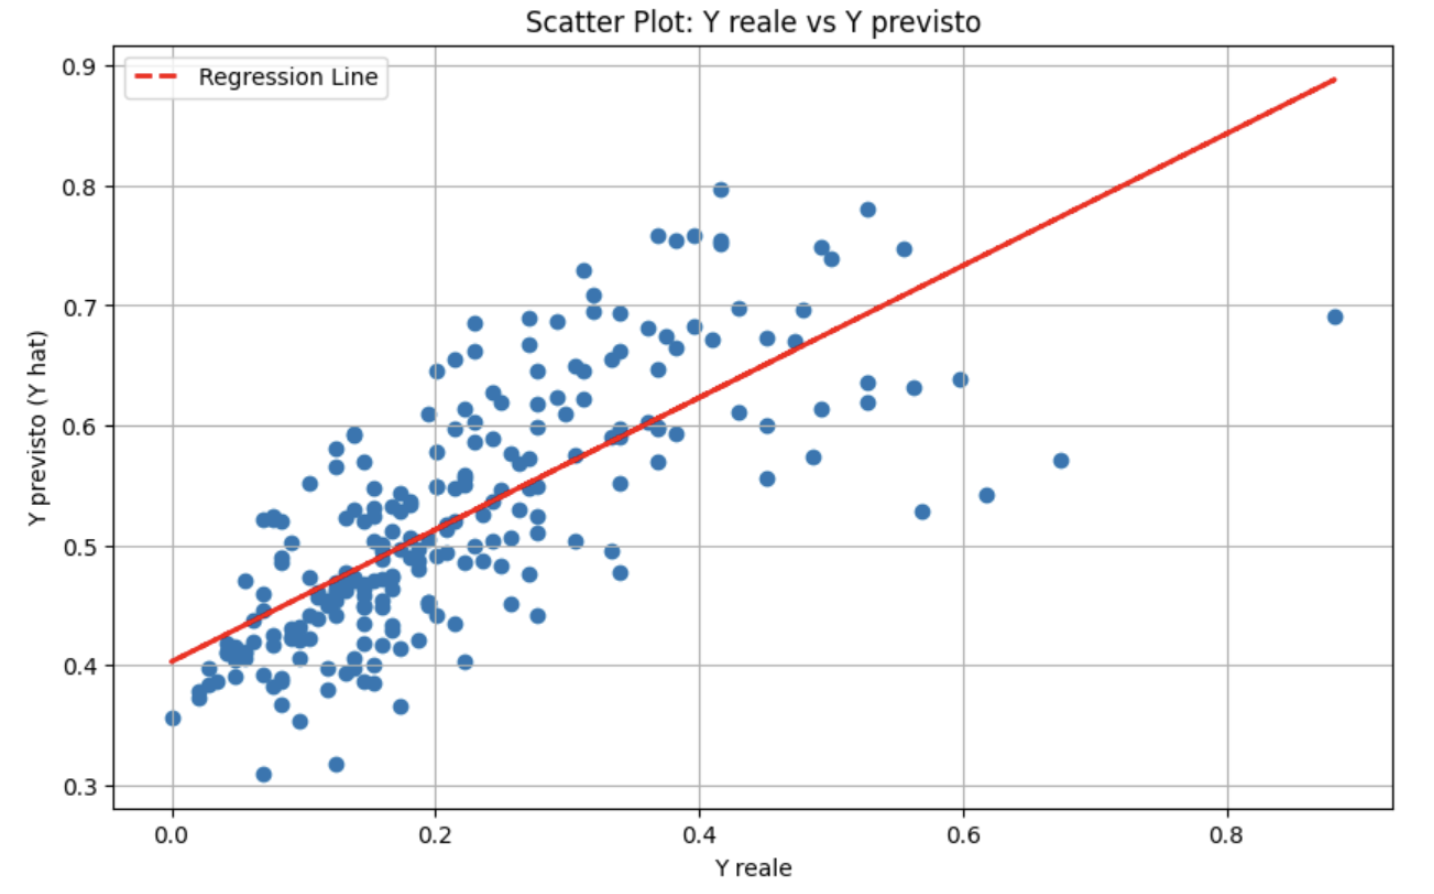
\includegraphics[scale=0.4]{Assets/iteration 1/lstm_it1_2.png}
        \caption{$\hat{y}$ vs. y\_real for LSTM for the second iteration}
        \label{fig:enter-label}
    \end{figure}
    \newpage

    \subsection{Results for the second iteration}

    The new starting parameters for the model are:
    \begin{itemize}
        \item  units\_hidden\_layer = [64, 128, 192, 256]
        \item learning\_rates = [0.001, 0.01, 0.1]
        \item num\_iterations\_range = [0, 5, 10, 20]
        \item num\_epochs\_range = [200, 250, 300, 350, 400]
    \end{itemize}
    
    Best Model Metrics training:
        \begin{itemize}
            \item Best MAE: 0.06
            \item Best R-squared (R2): 0.6
            \item Best RMSE: 0.08
        \end{itemize}
    
    Best Model Metrics:
    
        \begin{itemize}
            \item Best MAE: 0.06
            \item Best R-squared (R2): 0.6
            \item Best RMSE: 0.08
            \item Training Time for Best Model:  70.73 seconds
        \end{itemize}
    The LSTM model has been trained and evaluated with a range of hyperparameters, including varying units in the hidden layer, learning rates, number of iterations, and epochs.
    \\The training phase resulted in the best model achieving a remarkably low Mean Absolute Error (MAE) of 0.06, a high R-squared (R2) value of 0.6, and a small Root Mean Squared Error (RMSE) of 0.08.
    \\These metrics indicate that the LSTM architecture effectively captures the temporal dependencies in the data and exhibits strong predictive capabilities.
    \\The chosen hyperparameters for the best model include 250 epochs, no iterations, 256 units in the hidden layer, and a learning rate of 0.001.
    \\The training time for the best model is relatively higher compared to other models, at 70.73 seconds, likely due to the LSTM's inherent complexity and longer training duration.
    \\Overall, these results demonstrate the effectiveness of LSTM in modeling sequential data and its potential for achieving high predictive accuracy.
    
    \begin{figure}
        \centering
        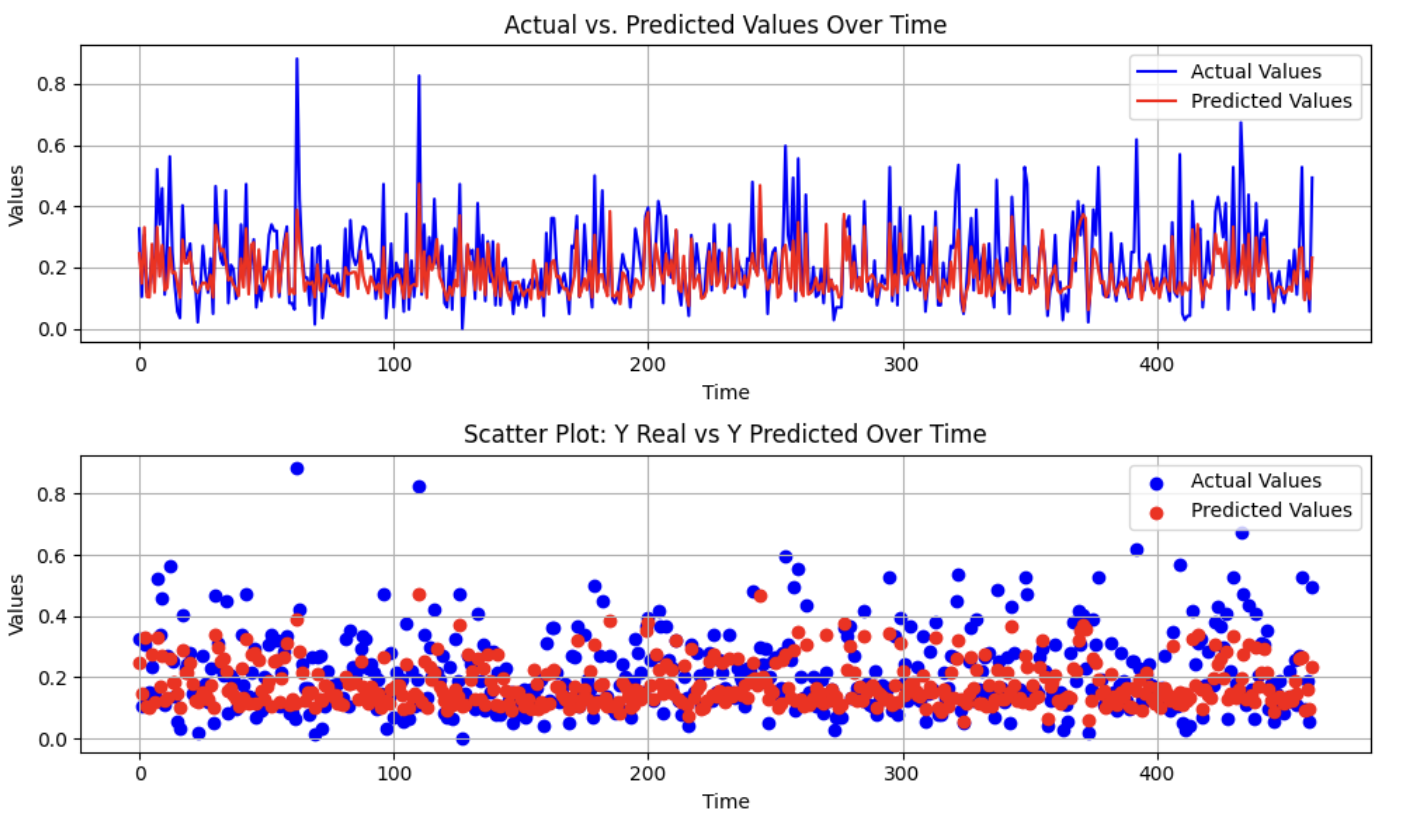
\includegraphics[scale=0.4]{Assets/iteration 2/lstm_it2_1.png}
        \caption{Time series for the LSTM result for the second iteration}
        \label{fig:enter-label}
    \end{figure}

    \begin{figure}
        \centering
        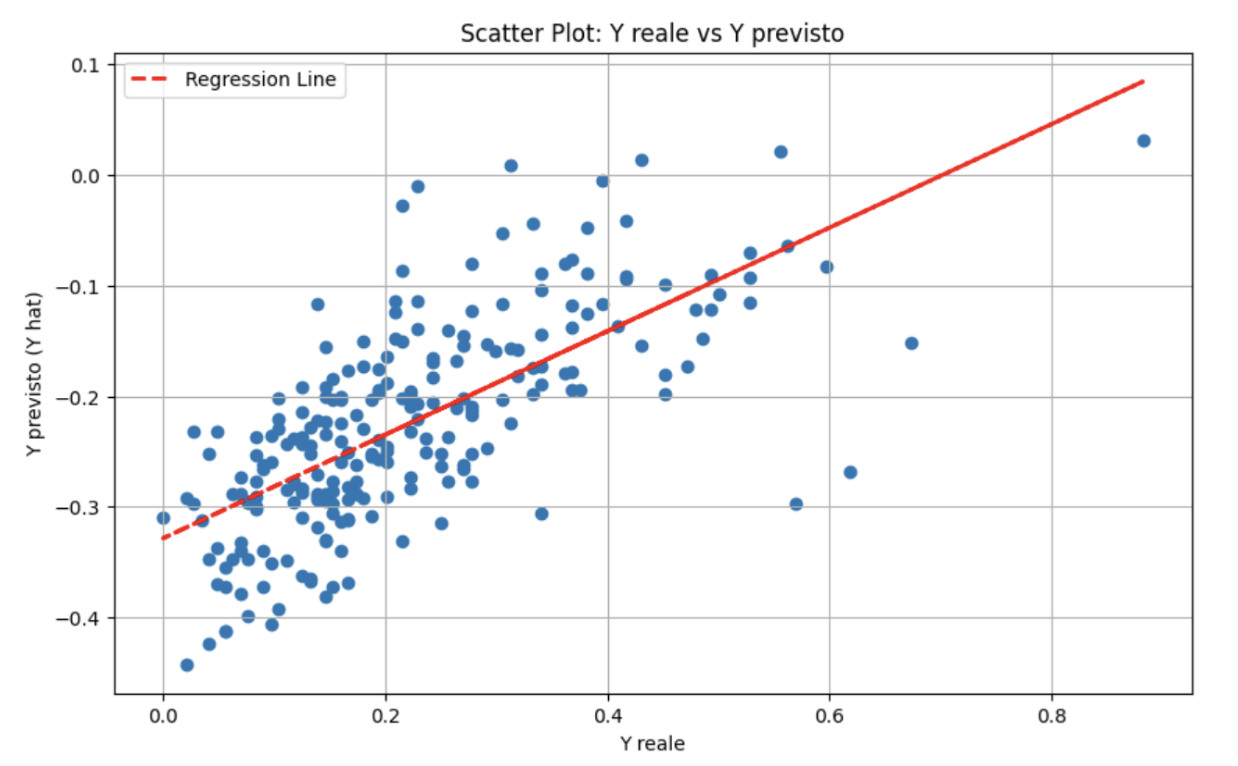
\includegraphics[scale=0.4]{Assets/iteration 2/lstm_it2_2.png}
        \caption{$\hat{y}$ vs. y\_real the LSTM model for the second iteration}
        \label{fig:enter-label}
    \end{figure}

    \newpage

\bibliography{bibliography} 

\end{document}
